\documentclass[11pt]{beamer}
\usetheme{default}
\usepackage[utf8]{inputenc}
\usepackage{amsmath}
\usepackage{amsfonts}
\usepackage{amssymb}
\usepackage{graphicx}

\author{Arne De Brabandere\\Robin Goots\\Ward Schodts\\Ronald Spilstijns}
\title{TaskMan: Iteratie 1}
%\setbeamercovered{transparent} 
\setbeamertemplate{navigation symbols}{} 
%\logo{} 
\institute{K.U. Leuven} 
\date{19/03/2015} 
%\subject{} 
\begin{document}

\begin{frame}
\titlepage
\end{frame}

%\begin{frame}
%\tableofcontents
%\end{frame}

% ONTWERP: LAGEN

\begin{frame}
\frametitle{Ontwerp: lagen}
\begin{itemize}
\item \textbf{Domein laag}
\begin{itemize}
	\item \textbf{`Echte' domein laag}\\Bevat klassen om projecten en taken bij te houden, ...
	\item \textbf{Use case controller laag}\\Bevat controllers die de stappen voor de use cases in de juiste volgorde uitvoeren en een interface die een gebruikersinterface klasse moet implementeren
\end{itemize}
\item \textbf{Presentatie laag}
\\Bevat de gebruikersinterface
\end{itemize}
\end{frame}

% ECHTE DOMEIN LAAG: overzicht

\begin{frame}
\frametitle{`Echte' domein laag: overzicht}
\begin{center}
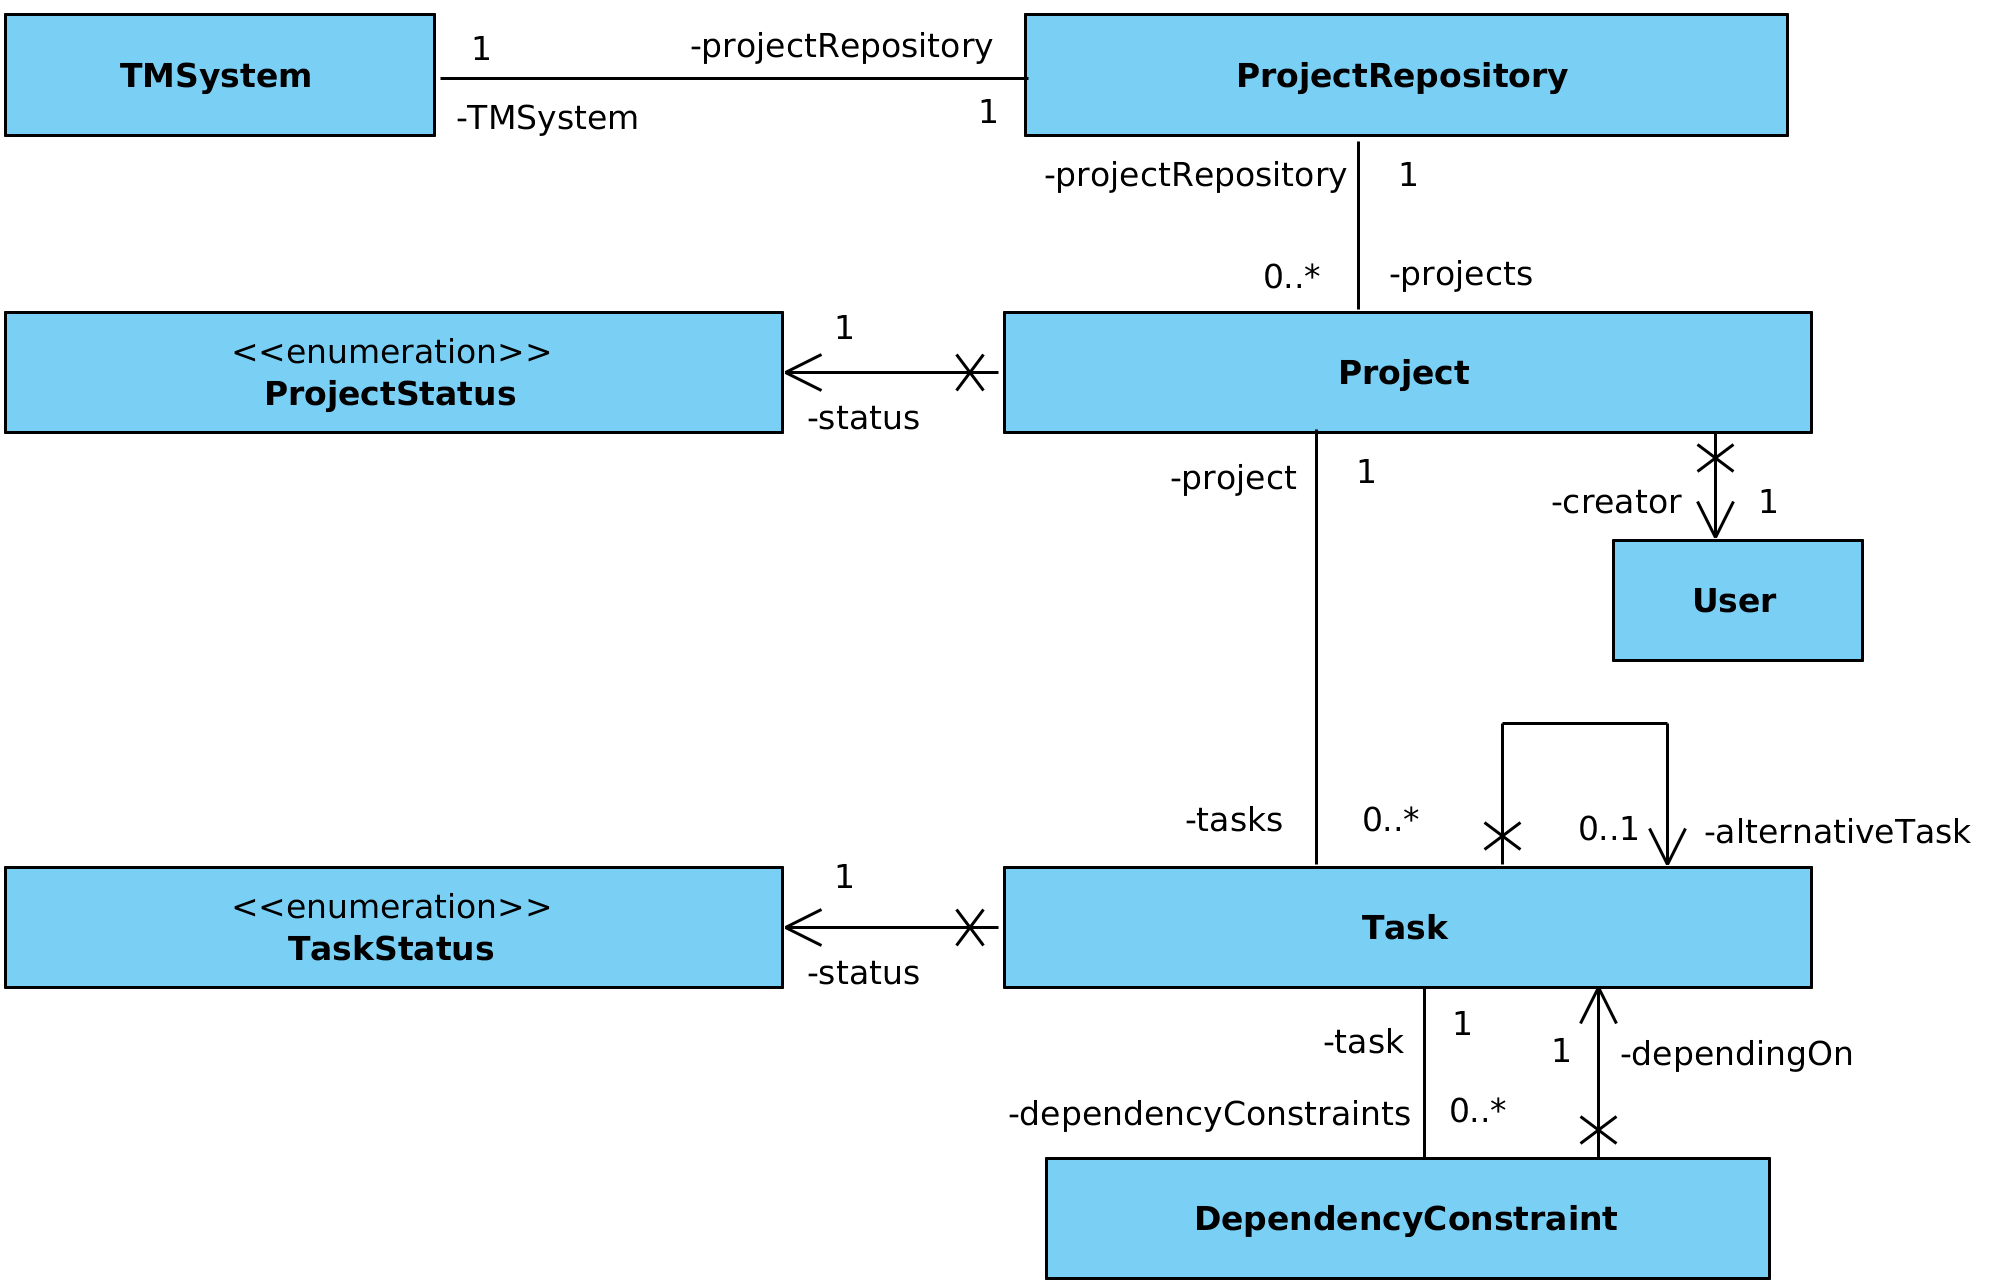
\includegraphics[width=\textwidth,height=0.8\textheight,keepaspectratio]{uml/proper_domain_overview.png}
\end{center}
\end{frame}

% USE CASE CONTROLLER LAAG: overzicht

\begin{frame}
\frametitle{Use case controller laag: overzicht}
\begin{center}
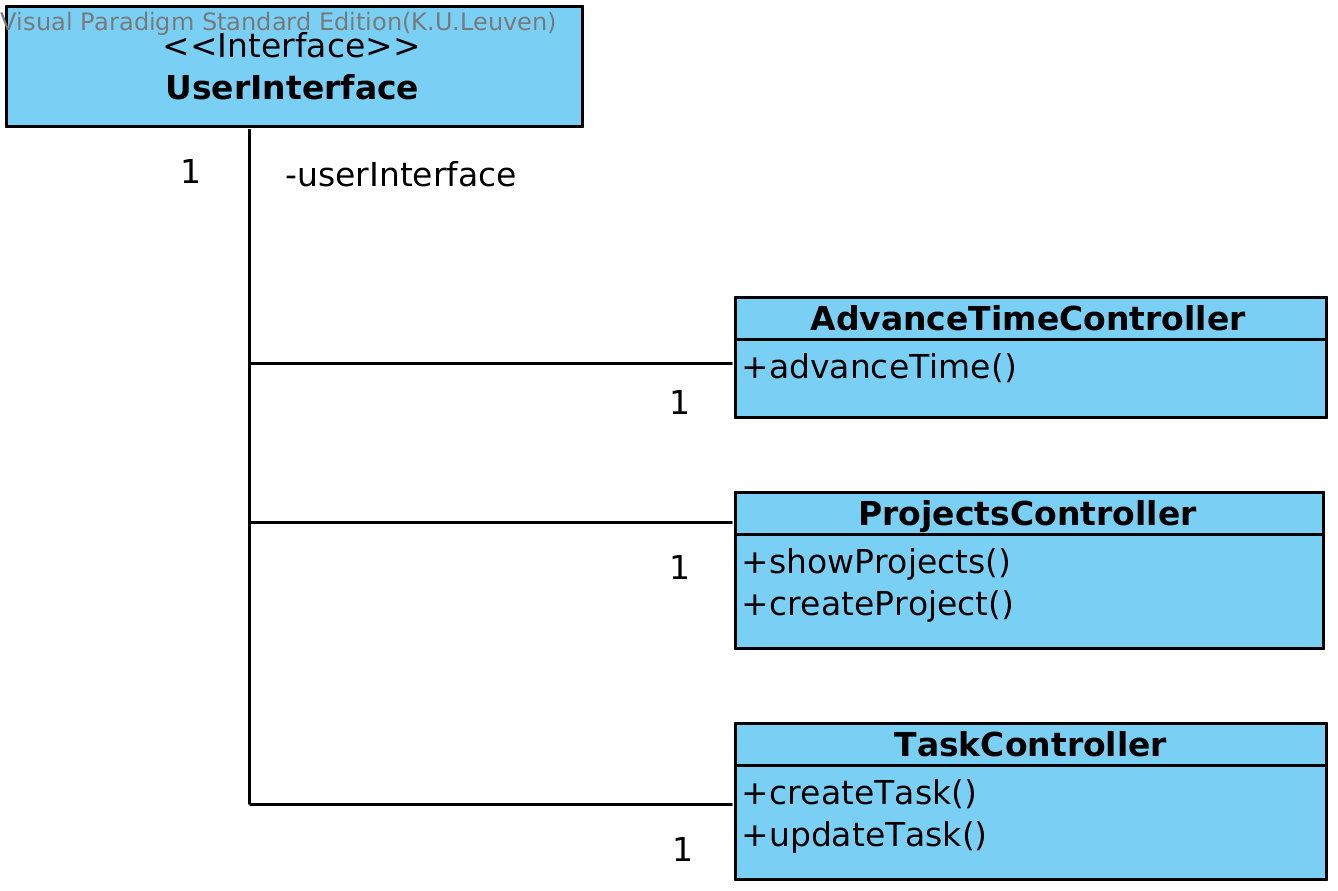
\includegraphics[width=\textwidth,height=0.8\textheight,keepaspectratio]{uml/use_case_controller_overview.png}
\end{center}
\end{frame}

% TODO: "overzicht" van presentatie laag

% TODO: verbinding tussen lagen laten zien (zorgen dat het diagram niet te uitgebreid wordt!)

% TODO: meer gedetaileerd ingaan op interessantere delen:
%	-> controllers?
%	-> dependency constraints + lusdetectie van dependencies?

% TODO: (samen met vorige slides over ontwerp) iets zeggen over uitbreidbaarheid

% TODO: kort iets zeggen over de testen (daarvan moeten we ook een demo geven!)

\end{document}